\documentclass[acmsmall]{acmart}
\usepackage{amsmath}
\usepackage{algorithm}
\usepackage{algorithmic}
\def\BibTeX{{\rm B\kern-.05em{\sc i\kern-.025em b}\kern-.08emT\kern-.1667em\lower.7ex\hbox{E}\kern-.125emX}}

\begin{document}

\title{Network of Favors in P2P cloud federation}

\author{Gustavo Diniz Monteiro}
\authornote{Responsible for research}
\email{gustavo.monteiro@ccc.ufcg.edu.br}
\email{gustavo.d.monteiro@icloud.com}
\affiliation{%
  \institution{Fedderal University of Campina Grande}
  \city{Campina Grande}
  \state{Paraiba}
  \country{Brazil}
}

\author{Francisco Brasileiro}
\authornote{Mentor}
\email{fubica@computacao.ufcg.edu.br}
\affiliation{%
  \institution{Fedderal University of Campina Grande}
  \city{Campina Grande}
  \state{Paraiba}
  \country{Brazil}
}

\begin{abstract}
Many organizations have extreme fluctuations of use, and during these peaks, they have to resort to public clouds to meet fleeting demand. The cost of such an action in itself can be expensive, which paired with possible sub-utilization organization's resources can generate high costs. The objective of this work is to present a tool to implement and incentive justice on resource sharing in P2P systems, initially using the direct reciprocity Network of Favors model. The direct reciprocity justice model that will be used for small and medium-sized networks, for scenarios where repeated peer interaction is most likely and where these organizations could meet their demand at peak times and offer favors in under utilization, with guarantee of protection against uncooperative members. In addition, the network focuses on being a lightweight solution, designed to be a pluggable and adaptable element to the provider, using first-hand knowledge gained by each member through direct interaction with other peers.
\end{abstract}

\keywords{federation, p2p networks, fairness}

\maketitle

\section{Introduction}
Organizations with varying demand patterns and utilization peaks often resort to public clouds (cf. ´´cloud bursting´´ \cite{cloudburst}) to meet unexpected or short-term needs, thus escaping failures in meeting business demands and quality of service goals.
However, outside of peak times, the resources of theses organizations may become inactive, which is a loss of efficiency.

Under these circumstances, selling this surplus of resources may be an interesting option for large private cloud providers, but not for smaller private providers.

One alternative that small and medium-sized private cloud providers may find advantageous is to collaboratively exchange idle capacity on a peer-to-peer (P2P) basis within a federation. In this case, each provider in the federation acts both as a resource provider (outside peak hours) and as a resource consumer (during peak times). In particular private cloud providers, because of the usually limited amount of own resources, would benefit greatly from this exchange\cite{fairness-benefices}, thus allowing them to access a larger pool of resources when local demand is too high and can not be met using only local resources and resources that simply do not exist locally.
The NOF\cite{nof} provider will work as a middleware for favors requests, and defining functional  interfaces  that  allow  support  to  different  federation  providers  and  justice  algorithms  for  Network  of  Favors  through  specific  modules  for  each  provider  and  chosen justice algorithm, which will act as adapters, aiming to be a platform configurable and adaptable to the model of justice and to the federation provider.

\section{Methodology}

This work is based on implementing and testing algorithms that will control peer-to-peer justice and global justice in a federation, as well as describe how the communication and allocation of resources will be as a software engineering work, implementing these algorithms in order to create interfaces and an generic architecture for the implementation of a network of favors in any federation with minimum effort.

\begin{figure}[h]
  \centering
  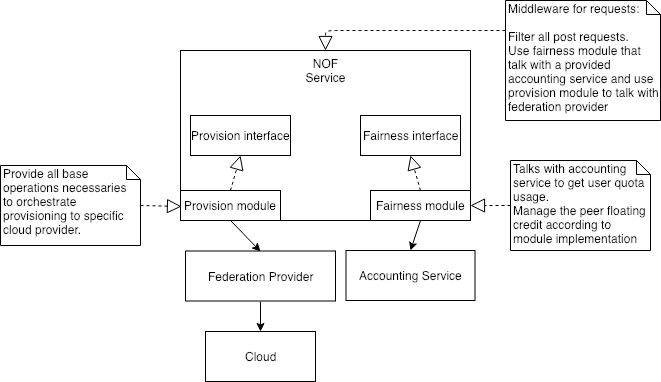
\includegraphics[width=\linewidth]{NOF-architecture-generic}
  \caption{NOF Architecture}
\end{figure}

The favors network architecture is defined so that all logic functions independently of the federation provider, where details of conversation with the provider and resource accounting are abstracted through proprietary drivers that must implement favour network interfaces.

The generic implementation of network of favors calculates its justice in two ways, the first of which is the relation between what a network peer provides resources and how much it consumes from it (global justice) and the relation between consumption and how much was given between two members of the federation (local justice).

\begin{math}
    provided == 0 \rightarrow fairness = -1
\end{math}


\begin{math}
    provided > 0 \rightarrow fairness = \dfrac{consumed}{provided}
\end{math}

In this context, the exchange of resources in the federation is defined in two parts, the first of which is defined as one peer can allocate a resource to another that is requesting.

\begin{algorithm}
\caption{Describe how to nof allocate a resource on local peer.}
\begin{algorithmic}
    \IF{requester has quota}
        \STATE success = createResource()
        \IF{success}
            \RETURN RESOURCE
        \ELSE
            \STATE members = getMemberWithSmallerQuota()
            \FOR{member in members}
                \FOR{resource in member.resources}
                    \STATE preempt(resource)
                    \STATE success = createResource()
                    \IF{success}
                        \RETURN RESOURCE
                    \ENDIF
                \ENDFOR
            \ENDFOR
            \STATE members = getMembersWithHigherDebts()
            \FOR{member in members}
                \STATE success = createRemote()
                \IF{success}
                    \RETURN RESOURCE
                \ENDIF
            \ENDFOR
            \RETURN ERROR
        \ENDIF
    \ELSE
        \RETURN ERROR
    \ENDIF
\end{algorithmic}
\end{algorithm}

The NOF works so that when a resource allocation request from another peer arrives, the NOF first checks if the peer has enough quota allocated for it to meet the request, if yes it is to create the resources, if not return a message describing the situation.
If the attempt to create the resource is successful, the information about the resource is returned to the peer, but if for a lack of resources the local peer has not been able to create resource, it will check if there are other registered peers that have a balance of local justice less than the peer owner of the request, and will then be filled one by one the resources of these members in order of which has less value of justice for the greater and each deletion will be tried again the creation of the  requested resource, if this operation was successfully will be returned the resource information.
If even with the fulfillment of these resources there is still not enough quota for creation of the resource then the refusal of cloudburst will be used.
Then will be listed again the members with less value of justice and will be passed sequentially to each one the request like a remote request.

In the second algorithm, remote creation, as is the allocation of resources to a remote request.

\begin{algorithm}
\caption{Describe how to nof allocate a resource from a remote request on local peer.}
\begin{algorithmic}
    \IF{has quota}
        \STATE success = createResource()
        \IF{success}
            \RETURN RESOURCE
        \ELSE
            \STATE members = getMemberWithSmallerQuota()
            \FOR{member in members}
                \FOR{resource in member.resources}
                    \STATE preempt(resource)
                    \STATE success = createResource()
                    \IF{success}
                        \RETURN RESOURCE
                    \ENDIF
                \ENDFOR
            \ENDFOR
            \RETURN ERROR
        \ENDIF
    \ELSE
        \RETURN ERROR
    \ENDIF
\end{algorithmic}
\end{algorithm}

When the NOF receives a remote request the creation of this resource will also change the fairness relationship between the peer receiving the request and the remote peer if it can attend the request. When receiving the request, it checks if the first recipient of that request has quota to meet that request, if it does try to create the resource, if it does not return to the original peer of the request that can not attend it.
If the creation failed due to insufficient reasons, the same cloudburst process of the local request algorithm is executed to free the resource and try again to fulfill the request, if it still could not create the resource, it will return to the original peer of the request that does not you can answer it.

\bibliographystyle{ACM-Reference-Format}
\bibliography{sample-base}

\end{document}
